\documentclass[11pt,]{article}
\usepackage[left=1in,top=1in,right=1in,bottom=1in]{geometry}
\newcommand*{\authorfont}{\fontfamily{phv}\selectfont}
\usepackage[]{mathpazo}
\usepackage{amsmath}
\usepackage{graphicx}
\usepackage{float}
  \usepackage[T1]{fontenc}
  \usepackage[utf8]{inputenc}

\newcommand{\red}[1]{\textcolor{red}{#1}}

\usepackage{abstract}
\renewcommand{\abstractname}{}    % clear the title
\renewcommand{\absnamepos}{empty} % originally center

\renewenvironment{abstract}
 {{%
    \setlength{\leftmargin}{0mm}
    \setlength{\rightmargin}{\leftmargin}%
  }%
  \relax}
 {\endlist}

\makeatletter
\def\@maketitle{%
  \newpage
%  \null
%  \vskip 2em%
%  \begin{center}%
  \let \footnote \thanks
    {\fontsize{18}{20}\selectfont\raggedright  \setlength{\parindent}{0pt} \@title \par}%
}
%\fi
\makeatother



\usepackage{color}
\usepackage{fancyvrb}
\newcommand{\VerbBar}{|}
\newcommand{\VERB}{\Verb[commandchars=\\\{\}]}
\DefineVerbatimEnvironment{Highlighting}{Verbatim}{commandchars=\\\{\}}
% Add ',fontsize=\small' for more characters per line
\usepackage{framed}
\definecolor{shadecolor}{RGB}{248,248,248}
\newenvironment{Shaded}{\begin{snugshade}}{\end{snugshade}}
\newcommand{\AlertTok}[1]{\textcolor[rgb]{0.94,0.16,0.16}{#1}}
\newcommand{\AnnotationTok}[1]{\textcolor[rgb]{0.56,0.35,0.01}{\textbf{\textit{#1}}}}
\newcommand{\AttributeTok}[1]{\textcolor[rgb]{0.77,0.63,0.00}{#1}}
\newcommand{\BaseNTok}[1]{\textcolor[rgb]{0.00,0.00,0.81}{#1}}
\newcommand{\BuiltInTok}[1]{#1}
\newcommand{\CharTok}[1]{\textcolor[rgb]{0.31,0.60,0.02}{#1}}
\newcommand{\CommentTok}[1]{\textcolor[rgb]{0.56,0.35,0.01}{\textit{#1}}}
\newcommand{\CommentVarTok}[1]{\textcolor[rgb]{0.56,0.35,0.01}{\textbf{\textit{#1}}}}
\newcommand{\ConstantTok}[1]{\textcolor[rgb]{0.00,0.00,0.00}{#1}}
\newcommand{\ControlFlowTok}[1]{\textcolor[rgb]{0.13,0.29,0.53}{\textbf{#1}}}
\newcommand{\DataTypeTok}[1]{\textcolor[rgb]{0.13,0.29,0.53}{#1}}
\newcommand{\DecValTok}[1]{\textcolor[rgb]{0.00,0.00,0.81}{#1}}
\newcommand{\DocumentationTok}[1]{\textcolor[rgb]{0.56,0.35,0.01}{\textbf{\textit{#1}}}}
\newcommand{\ErrorTok}[1]{\textcolor[rgb]{0.64,0.00,0.00}{\textbf{#1}}}
\newcommand{\ExtensionTok}[1]{#1}
\newcommand{\FloatTok}[1]{\textcolor[rgb]{0.00,0.00,0.81}{#1}}
\newcommand{\FunctionTok}[1]{\textcolor[rgb]{0.00,0.00,0.00}{#1}}
\newcommand{\ImportTok}[1]{#1}
\newcommand{\InformationTok}[1]{\textcolor[rgb]{0.56,0.35,0.01}{\textbf{\textit{#1}}}}
\newcommand{\KeywordTok}[1]{\textcolor[rgb]{0.13,0.29,0.53}{\textbf{#1}}}
\newcommand{\NormalTok}[1]{#1}
\newcommand{\OperatorTok}[1]{\textcolor[rgb]{0.81,0.36,0.00}{\textbf{#1}}}
\newcommand{\OtherTok}[1]{\textcolor[rgb]{0.56,0.35,0.01}{#1}}
\newcommand{\PreprocessorTok}[1]{\textcolor[rgb]{0.56,0.35,0.01}{\textit{#1}}}
\newcommand{\RegionMarkerTok}[1]{#1}
\newcommand{\SpecialCharTok}[1]{\textcolor[rgb]{0.00,0.00,0.00}{#1}}
\newcommand{\SpecialStringTok}[1]{\textcolor[rgb]{0.31,0.60,0.02}{#1}}
\newcommand{\StringTok}[1]{\textcolor[rgb]{0.31,0.60,0.02}{#1}}
\newcommand{\VariableTok}[1]{\textcolor[rgb]{0.00,0.00,0.00}{#1}}
\newcommand{\VerbatimStringTok}[1]{\textcolor[rgb]{0.31,0.60,0.02}{#1}}
\newcommand{\WarningTok}[1]{\textcolor[rgb]{0.56,0.35,0.01}{\textbf{\textit{#1}}}}
\usepackage{longtable,booktabs}

\usepackage{graphicx,grffile}
\makeatletter
\def\maxwidth{\ifdim\Gin@nat@width>\linewidth\linewidth\else\Gin@nat@width\fi}
\def\maxheight{\ifdim\Gin@nat@height>\textheight\textheight\else\Gin@nat@height\fi}
\makeatother
% Scale images if necessary, so that they will not overflow the page
% margins by default, and it is still possible to overwrite the defaults
% using explicit options in \includegraphics[width, height, ...]{}
\setkeys{Gin}{width=\maxwidth,height=\maxheight,keepaspectratio}

\title{HAZ in Uganda  }





\author{}

\setcounter{secnumdepth}{0}
\date{}

\usepackage{titlesec}

\titleformat*{\section}{\normalsize\bfseries}
\titleformat*{\subsection}{\normalsize\bfseries}
\titleformat*{\subsubsection}{\normalsize\itshape}
\titleformat*{\paragraph}{\normalsize\itshape}
\titleformat*{\subparagraph}{\normalsize\itshape}


\usepackage{natbib}
\bibliographystyle{apalike}
\usepackage[strings]{underscore} % protect underscores in most circumstances



\newtheorem{hypothesis}{Hypothesis}
\usepackage{setspace}

\makeatletter
\@ifpackageloaded{hyperref}{}{%
\ifxetex
  \PassOptionsToPackage{hyphens}{url}\usepackage[setpagesize=false, % page size defined by xetex
              unicode=false, % unicode breaks when used with xetex
              xetex]{hyperref}
\else
  \PassOptionsToPackage{hyphens}{url}\usepackage[unicode=true]{hyperref}
\fi
}

\@ifpackageloaded{color}{
    \PassOptionsToPackage{usenames,dvipsnames}{color}
}{%
    \usepackage[usenames,dvipsnames]{color}
}
\makeatother
\hypersetup{breaklinks=true,
            bookmarks=true,
            pdfauthor={},
             pdfkeywords = {},  
            pdftitle={HAZ in Uganda},
            colorlinks=true,
            citecolor=cyan,
            urlcolor=blue,
            linkcolor=magenta,
            pdfborder={0 0 0}}
\urlstyle{same}  % don't use monospace font for urls

% set default figure placement to htbp
\makeatletter
\def\fps@figure{htbp}
\makeatother

\usepackage[english]{babel}
\usepackage{booktabs}
\usepackage{longtable}
\usepackage{array}
\usepackage{multirow}
\usepackage[table]{xcolor}
\usepackage{wrapfig}
\usepackage{float}
\usepackage{colortbl}
\usepackage{pdflscape}
\usepackage{tabu}
\usepackage{threeparttable}
\usepackage{threeparttablex}
\usepackage[normalem]{ulem}
\usepackage{makecell}


% add tightlist ----------
\providecommand{\tightlist}{%
\setlength{\itemsep}{3pt}\setlength{\parskip}{0pt}}

\begin{document}
	
% \pagenumbering{arabic}% resets `page` counter to 1 
%
% \maketitle

{% \usefont{T1}{pnc}{m}{n}
\setlength{\parindent}{0pt}
\thispagestyle{plain}
{\fontsize{18}{20}\selectfont\raggedright 
\maketitle  % title \par  

}

{
   \vskip 13.5pt\relax \normalsize\fontsize{11}{12} 
 

}

}








\begin{abstract}

    \hbox{\vrule height .2pt width 39.14pc}

    \vskip 8.5pt % \small 

\noindent This report contains the R code and output of an analysis conducted on
HAZ with DHS data from Uganda


    \hbox{\vrule height .2pt width 39.14pc}


\end{abstract}


\vskip 6.5pt


\noindent  \begin{Shaded}
\begin{Highlighting}[]
\CommentTok{# Load all packages needed for the analysis}
\ControlFlowTok{if}\NormalTok{ (}\OperatorTok{!}\KeywordTok{require}\NormalTok{(}\StringTok{"pacman"}\NormalTok{)) }\KeywordTok{install.packages}\NormalTok{(}\StringTok{"pacman"}\NormalTok{)}
\NormalTok{pkgs =}\StringTok{ }\KeywordTok{c}\NormalTok{(}\StringTok{"sf"}\NormalTok{, }\StringTok{"dplyr"}\NormalTok{, }\StringTok{"PrevMap"}\NormalTok{, }\StringTok{"ggplot2"}\NormalTok{, }\StringTok{"tmap"}\NormalTok{)}
\NormalTok{pacman}\OperatorTok{::}\KeywordTok{p_load}\NormalTok{(pkgs, }\DataTypeTok{character.only =}\NormalTok{ T)}

\CommentTok{# Load external functions}
\KeywordTok{source}\NormalTok{(}\StringTok{"R/functions.R"}\NormalTok{)}
\end{Highlighting}
\end{Shaded}

\hypertarget{data-cleaning}{%
\section{Data cleaning}\label{data-cleaning}}

Coordinates were converted from lat/long WGS84 to UTM zone 35N (in Km).
10 clusters have been removed from the analysis because lat and long was
not available. In the original dataset the HAZ ranges from a minimum of
-6 to a maximum of 99.98. A total of 22 individuals were removed because
an extreme value of HAZ was reporterd (equal to 99.98). Other 26
individuals have been removed because either HAZ or vitamin A was not
recorded.

\begin{Shaded}
\begin{Highlighting}[]
\CommentTok{# Load HAZ data}
\NormalTok{haz <-}\StringTok{ }\NormalTok{readr}\OperatorTok{::}\KeywordTok{read_csv}\NormalTok{(}\StringTok{"data/stunting_ug.csv"}\NormalTok{)}

\CommentTok{# Remove missing LAT LONG (some entries have 0 values)}
\CommentTok{# Remove also non admissable values for HAZ (== 99.98 and missing values)}
\CommentTok{# Remove individuals with missing vitamin A}
\NormalTok{haz <-}\StringTok{ }\NormalTok{haz }\OperatorTok\StringTok{ }
\StringTok{  }\KeywordTok{filter}\NormalTok{(LONGNUM }\OperatorTok{!=}\StringTok{ }\DecValTok{0}\NormalTok{, }\OperatorTok{!}\KeywordTok{is.na}\NormalTok{(HAZ), HAZ }\OperatorTok{<}\StringTok{ }\DecValTok{50}\NormalTok{, }\OperatorTok{!}\KeywordTok{is.na}\NormalTok{(VitaminA_microgram_per_Ml))}

\CommentTok{# Convert the LAT LONG coordinates to UTM (km) EPSSG: 32365}
\NormalTok{crs_utm_km <-}\StringTok{ }\KeywordTok{epsgKM}\NormalTok{(}\DecValTok{32635}\NormalTok{)}
\NormalTok{haz_sp <-}\StringTok{ }\NormalTok{haz }\OperatorTok\StringTok{ }
\StringTok{  }\KeywordTok{st_as_sf}\NormalTok{(}\DataTypeTok{coords =} \KeywordTok{c}\NormalTok{(}\StringTok{"LONGNUM"}\NormalTok{, }\StringTok{"LATNUM"}\NormalTok{), }\DataTypeTok{crs =} \DecValTok{4326}\NormalTok{) }\OperatorTok\StringTok{ }
\StringTok{  }\KeywordTok{st_transform}\NormalTok{(}\DataTypeTok{crs =}\NormalTok{ crs_utm_km)}

\CommentTok{# For a quick interactive view of the data run the following line of code}
\CommentTok{# mapview::mapview(haz_sp)}

\CommentTok{# Add two new columns with the coordinates in UTM (km)}
\NormalTok{haz[, }\KeywordTok{c}\NormalTok{(}\StringTok{"utm_x"}\NormalTok{, }\StringTok{"utm_y"}\NormalTok{)] <-}\StringTok{ }\KeywordTok{st_coordinates}\NormalTok{(haz_sp)}

\CommentTok{# Transform vitamin A to the log scale}
\NormalTok{haz}\OperatorTok{$}\NormalTok{log_VITA <-}\StringTok{ }\KeywordTok{log}\NormalTok{(haz}\OperatorTok{$}\NormalTok{VitaminA_microgram_per_Ml)}

\CommentTok{# Select only the columns relevant for the anlysis}
\NormalTok{haz <-}\StringTok{ }\NormalTok{haz }\OperatorTok\StringTok{ }
\StringTok{  }\NormalTok{dplyr}\OperatorTok{::}\KeywordTok{select}\NormalTok{(HAZ, log_VITA, }\DataTypeTok{agem =}\NormalTok{ Age_Month, }
\NormalTok{                Cluster_ID, utm_x, utm_y) }

\CommentTok{# Check if there are any missing values}
\NormalTok{missing <-}\StringTok{ }\KeywordTok{sapply}\NormalTok{(haz, }\ControlFlowTok{function}\NormalTok{(x) }\KeywordTok{sum}\NormalTok{(}\KeywordTok{is.na}\NormalTok{(x)))}
\NormalTok{knitr}\OperatorTok{::}\KeywordTok{kable}\NormalTok{(missing, }\DataTypeTok{col.names =} \StringTok{"Number of missing"}\NormalTok{)}
\end{Highlighting}
\end{Shaded}

\begin{longtable}[]{@{}lr@{}}
\toprule
& Number of missing\tabularnewline
\midrule
\endhead
HAZ & 0\tabularnewline
log\_VITA & 0\tabularnewline
agem & 0\tabularnewline
Cluster\_ID & 0\tabularnewline
utm\_x & 0\tabularnewline
utm\_y & 0\tabularnewline
\bottomrule
\end{longtable}

\hypertarget{raster-covariates}{%
\section{Raster covariates}\label{raster-covariates}}

\begin{Shaded}
\begin{Highlighting}[]
\CommentTok{# Load shapefile for Uganda}
\NormalTok{uga <-}\StringTok{ }\KeywordTok{st_read}\NormalTok{(}\StringTok{"data/geodata/gadm36_UGA.gpkg"}\NormalTok{, }\DataTypeTok{layer =} \StringTok{"gadm36_UGA_0"}\NormalTok{)}
\end{Highlighting}
\end{Shaded}

\begin{verbatim}
## Reading layer `gadm36_UGA_0' from data source `/home/claudio/Dropbox/chicas/HAZ_uganda/data/geodata/gadm36_UGA.gpkg' using driver `GPKG'
## Simple feature collection with 1 feature and 2 fields
## geometry type:  POLYGON
## dimension:      XY
## bbox:           xmin: 29.5715 ymin: -1.48214 xmax: 35.00027 ymax: 4.234466
## epsg (SRID):    4326
## proj4string:    +proj=longlat +datum=WGS84 +no_defs
\end{verbatim}

\begin{Shaded}
\begin{Highlighting}[]
\CommentTok{# Convert to the reference system of the points}
\NormalTok{uga <-}\StringTok{ }\KeywordTok{st_transform}\NormalTok{(uga, }\DataTypeTok{crs =}\NormalTok{ crs_utm_km)}

\CommentTok{# Load population raster}
\NormalTok{pop <-}\StringTok{ }\KeywordTok{raster}\NormalTok{(}\StringTok{"data/geodata/pop2016_100m.tif"}\NormalTok{)}

\CommentTok{# Create prediction grid}
\NormalTok{pred <-}\StringTok{ }\KeywordTok{create_grid}\NormalTok{(}\DataTypeTok{resolution =} \DecValTok{5}\NormalTok{, }\DataTypeTok{study_area =}\NormalTok{ uga, }\DataTypeTok{pop =}\NormalTok{ pop, }
                    \DataTypeTok{cutoff =} \DecValTok{0}\NormalTok{)}

\CommentTok{# Load raster covariates and align them to the prediction grid}
\NormalTok{elevation <-}\StringTok{ }\KeywordTok{raster}\NormalTok{(}\StringTok{"data/geodata/elevation2000_100m.tif"}\NormalTok{)}
\NormalTok{slope <-}\StringTok{ }\KeywordTok{raster}\NormalTok{(}\StringTok{"data/geodata/slope2000_100m.tif"}\NormalTok{)}
\NormalTok{evi <-}\StringTok{ }\KeywordTok{raster}\NormalTok{(}\StringTok{"data/geodata/evi2016_1km.tif"}\NormalTok{)}

\NormalTok{elevation <-}\StringTok{ }\KeywordTok{align_raster}\NormalTok{(}\DataTypeTok{pred =}\NormalTok{ pred}\OperatorTok{$}\NormalTok{raster, }\DataTypeTok{cov =}\NormalTok{ elevation)}
\NormalTok{slope <-}\StringTok{ }\KeywordTok{align_raster}\NormalTok{(}\DataTypeTok{pred =}\NormalTok{ pred}\OperatorTok{$}\NormalTok{raster, }\DataTypeTok{cov =}\NormalTok{ slope)}
\NormalTok{evi <-}\StringTok{ }\KeywordTok{align_raster}\NormalTok{(}\DataTypeTok{pred =}\NormalTok{ pred}\OperatorTok{$}\NormalTok{raster, }\DataTypeTok{cov =}\NormalTok{ evi)}

\CommentTok{# Stack all the raster covariates together}
\NormalTok{covariates <-}\StringTok{ }\KeywordTok{stack}\NormalTok{(elevation, slope, evi)}

\CommentTok{# Extract them at the observed locations}
\NormalTok{cov_obs  <-}\StringTok{ }\KeywordTok{extract}\NormalTok{(covariates, haz[, }\KeywordTok{c}\NormalTok{(}\StringTok{"utm_x"}\NormalTok{, }\StringTok{"utm_y"}\NormalTok{)])}

\CommentTok{# Fill NA}
\CommentTok{# idna <- which(is.na(cov_obs[, 1]))}
\CommentTok{# cov_obs[idna, ] <- extract(covariates, haz[idna, c("utm_x", "utm_y")],}
\CommentTok{#                            small = T, buffer = 5)}

\NormalTok{haz[, }\KeywordTok{c}\NormalTok{(}\StringTok{"elevation"}\NormalTok{, }\StringTok{"slope"}\NormalTok{, }\StringTok{"evi"}\NormalTok{)] <-}\StringTok{ }\NormalTok{cov_obs}

\CommentTok{# Remove NA}
\NormalTok{haz <-}\StringTok{ }\NormalTok{haz[}\OperatorTok{!}\KeywordTok{is.na}\NormalTok{(haz}\OperatorTok{$}\NormalTok{elevation), ]}
\end{Highlighting}
\end{Shaded}

\hypertarget{relationship-between-haz-and-individual-variables}{%
\section{Relationship between HAZ and individual
variables}\label{relationship-between-haz-and-individual-variables}}

Let's have a look at the relationship between HAZ scores and individual
levle variables. If this relatioship turns out to be non-linear we will
accomodate for it. From \autoref{fig:individual_rel} we can't really see
a clear relationship between vitamin A and HAZ. For age, it looks like
there is a decrease in HAZ until approximately 20 months and then no
relationship.

\begin{Shaded}
\begin{Highlighting}[]
\NormalTok{haz }\OperatorTok\StringTok{ }
\StringTok{  }\NormalTok{dplyr}\OperatorTok{::}\KeywordTok{select}\NormalTok{(HAZ, log_VITA, agem) }\OperatorTok\StringTok{ }
\StringTok{  }\NormalTok{tidyr}\OperatorTok{::}\KeywordTok{gather}\NormalTok{(}\DataTypeTok{key =} \StringTok{"variable"}\NormalTok{, }\DataTypeTok{value =} \StringTok{"value"}\NormalTok{, }\OperatorTok{-}\NormalTok{HAZ) }\OperatorTok\StringTok{ }
\StringTok{  }\KeywordTok{ggplot}\NormalTok{(}\KeywordTok{aes}\NormalTok{(}\DataTypeTok{x =}\NormalTok{ value, }\DataTypeTok{y =}\NormalTok{ HAZ)) }\OperatorTok{+}
\StringTok{  }\KeywordTok{geom_point}\NormalTok{(}\DataTypeTok{shape =} \DecValTok{21}\NormalTok{, }\DataTypeTok{fill =} \StringTok{"black"}\NormalTok{, }\DataTypeTok{alpha =} \FloatTok{.3}\NormalTok{, }\DataTypeTok{size =} \FloatTok{.5}\NormalTok{) }\OperatorTok{+}
\StringTok{  }\KeywordTok{geom_smooth}\NormalTok{(}\DataTypeTok{method =} \StringTok{"gam"}\NormalTok{, }\DataTypeTok{formula =}\NormalTok{ y }\OperatorTok{~}\StringTok{ }\KeywordTok{s}\NormalTok{(x), }\DataTypeTok{size =} \FloatTok{.5}\NormalTok{) }\OperatorTok{+}
\StringTok{  }\KeywordTok{facet_wrap}\NormalTok{(}\OperatorTok{~}\StringTok{ }\NormalTok{variable, }\DataTypeTok{scales =} \StringTok{"free"}\NormalTok{, }
             \DataTypeTok{labeller =} \KeywordTok{labeller}\NormalTok{(}\DataTypeTok{variable =} \ControlFlowTok{function}\NormalTok{(x) }\KeywordTok{c}\NormalTok{(}\StringTok{"Age (months)"}\NormalTok{, }\StringTok{"Vitamin A (log)"}\NormalTok{))) }\OperatorTok{+}
\StringTok{  }\KeywordTok{labs}\NormalTok{(}\DataTypeTok{y =} \StringTok{"HAZ"}\NormalTok{) }\OperatorTok{+}
\StringTok{  }\KeywordTok{theme_bw}\NormalTok{()}
\end{Highlighting}
\end{Shaded}

\begin{figure}[H]

{\centering 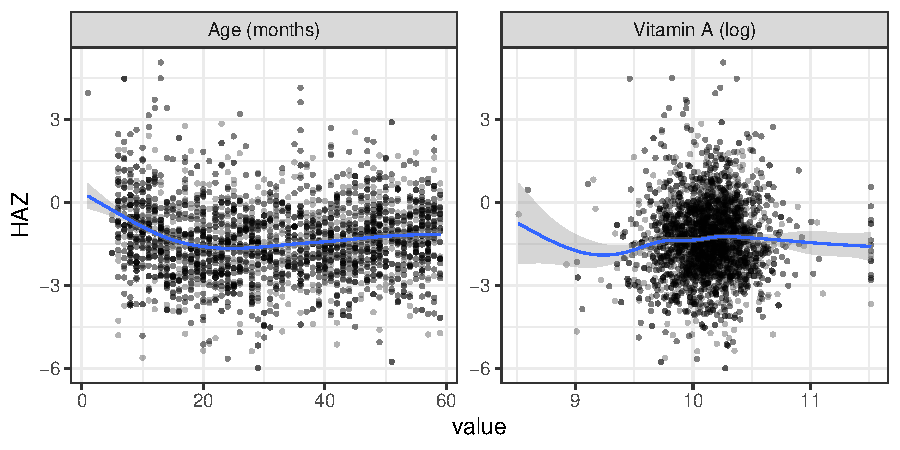
\includegraphics{skeleton_files/figure-latex/individual_rel-1} 

}

\caption{Scatterplot of the relationship between age (in month) and vitamin A (log scale) with HAZ. The blue line shows the fit of a GAM model (with a thin plate regression spline).}\label{fig:individual_rel}
\end{figure}

\begin{Shaded}
\begin{Highlighting}[]
\CommentTok{# Compare different models for HAZ vs. age}
\KeywordTok{library}\NormalTok{(splines)}
\KeywordTok{ggplot}\NormalTok{(haz, }\KeywordTok{aes}\NormalTok{(}\DataTypeTok{x =}\NormalTok{ agem, }\DataTypeTok{y =}\NormalTok{ HAZ)) }\OperatorTok{+}
\StringTok{  }\KeywordTok{geom_point}\NormalTok{(}\DataTypeTok{shape =} \DecValTok{21}\NormalTok{, }\DataTypeTok{fill =} \StringTok{"black"}\NormalTok{, }\DataTypeTok{alpha =} \FloatTok{.3}\NormalTok{, }\DataTypeTok{size =} \DecValTok{1}\NormalTok{) }\OperatorTok{+}
\StringTok{  }\KeywordTok{geom_smooth}\NormalTok{(}\DataTypeTok{method =} \StringTok{"gam"}\NormalTok{, }\DataTypeTok{formula =}\NormalTok{ y }\OperatorTok{~}\StringTok{ }\KeywordTok{s}\NormalTok{(x), }\KeywordTok{aes}\NormalTok{(}\DataTypeTok{col =} \StringTok{"GAM"}\NormalTok{, }\DataTypeTok{fill =} \StringTok{"GAM"}\NormalTok{),}
              \DataTypeTok{size =} \DecValTok{1}\NormalTok{) }\OperatorTok{+}
\StringTok{  }\KeywordTok{geom_smooth}\NormalTok{(}\DataTypeTok{method =} \StringTok{"lm"}\NormalTok{, }\DataTypeTok{formula =}\NormalTok{ y }\OperatorTok{~}\StringTok{ }\KeywordTok{bs}\NormalTok{(x, }\DataTypeTok{knots =} \FloatTok{17.84}\NormalTok{, }\DataTypeTok{degree =} \DecValTok{1}\NormalTok{),}
              \KeywordTok{aes}\NormalTok{(}\DataTypeTok{col =} \StringTok{"LINEAR"}\NormalTok{, }\DataTypeTok{fill =} \StringTok{"LINEAR"}\NormalTok{), }\DataTypeTok{size =} \DecValTok{1}\NormalTok{) }\OperatorTok{+}
\StringTok{  }\KeywordTok{labs}\NormalTok{(}\DataTypeTok{x =} \StringTok{"Age (months)"}\NormalTok{, }\DataTypeTok{y =} \StringTok{"HAZ"}\NormalTok{) }\OperatorTok{+}
\StringTok{  }\KeywordTok{scale_color_brewer}\NormalTok{(}\StringTok{"Model fit"}\NormalTok{, }\DataTypeTok{type =} \StringTok{"q"}\NormalTok{, }\DataTypeTok{palette =} \DecValTok{6}\NormalTok{) }\OperatorTok{+}
\StringTok{  }\KeywordTok{scale_fill_brewer}\NormalTok{(}\StringTok{"Model fit"}\NormalTok{, }\DataTypeTok{type =} \StringTok{"q"}\NormalTok{, }\DataTypeTok{palette =} \DecValTok{6}\NormalTok{) }\OperatorTok{+}
\StringTok{  }\KeywordTok{theme_bw}\NormalTok{()}
\end{Highlighting}
\end{Shaded}

\begin{figure}[H]

{\centering 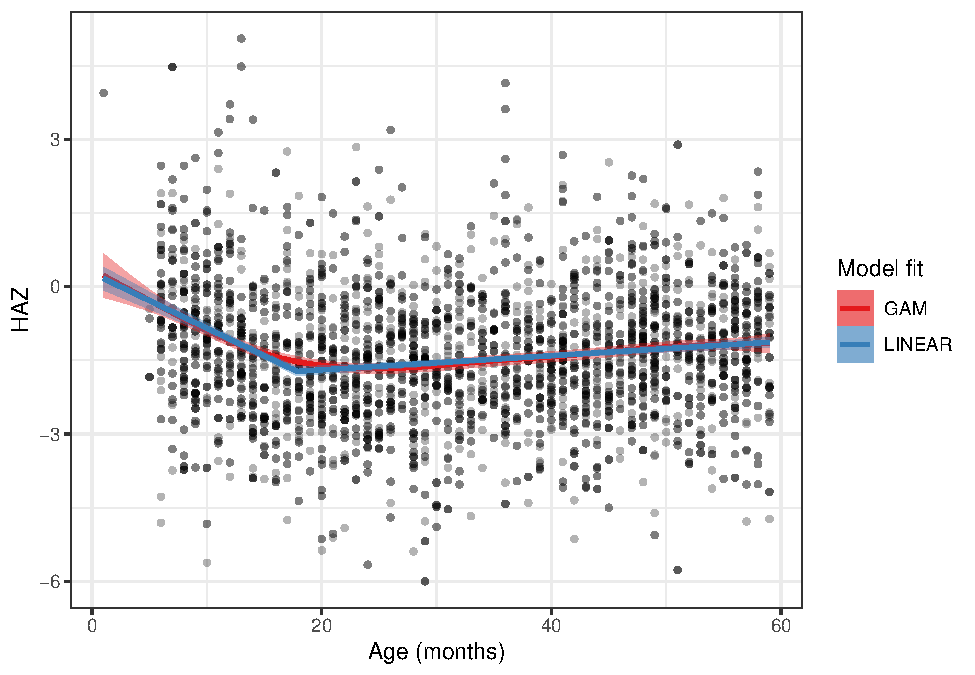
\includegraphics{skeleton_files/figure-latex/agevshaz-1} 

}

\caption{Comparison of the fit of a GAM and piece-wise linear regression to age and HAZ.}\label{fig:agevshaz}
\end{figure}

\begin{Shaded}
\begin{Highlighting}[]
\CommentTok{# Find optimal break point}
\CommentTok{# fcost <- function(param) \{}
\CommentTok{#   fit <- lm(HAZ ~ bs(agem, knots = param, degree = 1), data = haz)}
\CommentTok{#   aic <- AIC(fit)}
\CommentTok{#   return(aic)}
\CommentTok{# \}}
\CommentTok{# }
\CommentTok{# optim(par= 0, fn = fcost, method = "Brent", lower = -2, upper = 2)}
\end{Highlighting}
\end{Shaded}

\hypertarget{non-spatial-model}{%
\section{Non-spatial model}\label{non-spatial-model}}

Here we fit the following linear mixed model to the HAZ data
\begin{equation}
Y_j(x_i)=\alpha+\gamma d_{ij} + \beta d(x_i) + U_{i} + Z_{ij}
\end{equation} where \(Y_j(x_i)\) denotes the HAZ of the \(j\)th child
at cluster location \(x_i\), \(d_{ij}\) is a vector of individual level
covariates (age and vitamin A), \(d(x_i)\) is the vector of spatially
referenced environmental variables (elevation, slope and EVI). \(U_{i}\)
and \(Z_{ij}\) are two set of independent normally distributed random
effects who capture cluster level and individual level variation
respectively. We use the estimated \(\hat{U_i}\) to calculate the
variogram and check the presence of residual spatial variation.

\begin{Shaded}
\begin{Highlighting}[]
\CommentTok{# Load package to fit Mixed Model}
\KeywordTok{library}\NormalTok{(lme4)}

\CommentTok{# Before fitting this type of models it is alway a good idea to rescale the}
\CommentTok{# numeric variables (substract the mean and divide by the standard devation)}
\CommentTok{# to avoid problem of convergence}

\CommentTok{# Scale the numeric covariates}
\CommentTok{# num_covariates <- c("agem", "log_VITA", "elevation", "slope", "evi")}
\CommentTok{# haz[, num_covariates] <- scale(haz[, num_covariates])}

\CommentTok{# Create new ID for clusters}
\NormalTok{haz <-}\StringTok{ }\KeywordTok{as.data.frame}\NormalTok{(haz)}
\NormalTok{haz}\OperatorTok{$}\NormalTok{ID <-}\StringTok{ }\KeywordTok{create.ID.coords}\NormalTok{(}\DataTypeTok{data =}\NormalTok{ haz, }\OperatorTok{~}\StringTok{ }\NormalTok{utm_x }\OperatorTok{+}\StringTok{ }\NormalTok{utm_y)}
\NormalTok{haz}\OperatorTok{$}\NormalTok{Cluster_ID <-}\StringTok{ }\OtherTok{NULL}

\CommentTok{# Formula}
\NormalTok{f <-}\StringTok{ }\NormalTok{HAZ }\OperatorTok{~}\StringTok{ }\NormalTok{agem }\OperatorTok{+}\StringTok{ }\KeywordTok{I}\NormalTok{((agem }\OperatorTok{-}\StringTok{ }\FloatTok{17.84}\NormalTok{) }\OperatorTok{*}\StringTok{ }\NormalTok{(agem }\OperatorTok{>}\StringTok{ }\FloatTok{17.84}\NormalTok{)) }\OperatorTok{+}\StringTok{ }\NormalTok{log_VITA }\OperatorTok{+}\StringTok{ }
\StringTok{  }\NormalTok{elevation }\OperatorTok{+}\StringTok{ }\NormalTok{slope }\OperatorTok{+}\StringTok{ }\NormalTok{evi}

\CommentTok{# Formula with cluster level random effects}
\NormalTok{fcluster <-}\StringTok{ }\KeywordTok{update}\NormalTok{(f, }\OperatorTok{~}\StringTok{ }\NormalTok{. }\OperatorTok{+}\StringTok{ }\NormalTok{(}\DecValTok{1}\OperatorTok{|}\NormalTok{ID))}

\CommentTok{# Fit the model in equation (1)}
\NormalTok{fit <-}\StringTok{ }\KeywordTok{lmer}\NormalTok{(}\DataTypeTok{formula =}\NormalTok{ fcluster, }\DataTypeTok{data =}\NormalTok{ haz)}

\CommentTok{# Generate summary of the model}
\KeywordTok{summary}\NormalTok{(fit)}
\end{Highlighting}
\end{Shaded}

\begin{verbatim}
## Linear mixed model fit by REML ['lmerMod']
## Formula: HAZ ~ agem + I((agem - 17.84) * (agem > 17.84)) + log_VITA +  
##     elevation + slope + evi + (1 | ID)
##    Data: haz
## 
## REML criterion at convergence: 12146.7
## 
## Scaled residuals: 
##     Min      1Q  Median      3Q     Max 
## -3.2402 -0.6017 -0.0323  0.5392  4.3494 
## 
## Random effects:
##  Groups   Name        Variance Std.Dev.
##  ID       (Intercept) 0.5068   0.7119  
##  Residual             1.3913   1.1795  
## Number of obs: 3623, groups:  ID, 599
## 
## Fixed effects:
##                                      Estimate Std. Error t value
## (Intercept)                        -9.074e-01  9.199e-01  -0.986
## agem                               -1.068e-01  7.969e-03 -13.407
## I((agem - 17.84) * (agem > 17.84))  1.209e-01  9.071e-03  13.328
## log_VITA                            1.499e-01  8.572e-02   1.748
## elevation                          -1.753e-05  2.525e-04  -0.069
## slope                              -4.246e-02  1.870e-02  -2.271
## evi                                -5.942e-01  4.936e-01  -1.204
## 
## Correlation of Fixed Effects:
##             (Intr) agem   I-1*(>1 l_VITA elevtn slope 
## agem        -0.126                                    
## I((-17.*(>1  0.121 -0.986                             
## log_VITA    -0.929 -0.005  0.002                      
## elevation   -0.263  0.010 -0.009  -0.034              
## slope        0.246 -0.014  0.012  -0.004 -0.759       
## evi         -0.186  0.010 -0.010  -0.017  0.098 -0.331
## fit warnings:
## Some predictor variables are on very different scales: consider rescaling
\end{verbatim}

\begin{Shaded}
\begin{Highlighting}[]
\CommentTok{# Extract the random effects at cluster level U_i}
\NormalTok{reff <-}\StringTok{ }\KeywordTok{ranef}\NormalTok{(fit)}\OperatorTok{$}\NormalTok{ID}\OperatorTok{$}\StringTok{`}\DataTypeTok{(Intercept)}\StringTok{`}

\CommentTok{# Extract coordinates for each cluster}
\NormalTok{coords <-}\StringTok{ }\NormalTok{haz }\OperatorTok
\StringTok{  }\KeywordTok{distinct}\NormalTok{(ID, utm_x, utm_y) }\OperatorTok\StringTok{ }
\StringTok{  }\KeywordTok{arrange}\NormalTok{(ID) }\OperatorTok\StringTok{ }
\StringTok{  }\NormalTok{dplyr}\OperatorTok{::}\KeywordTok{select}\NormalTok{(utm_x, utm_y)}

\CommentTok{# Load ggvario function}
\KeywordTok{ggvario}\NormalTok{(}\DataTypeTok{coords =}\NormalTok{ coords, }\DataTypeTok{data =}\NormalTok{ reff, }\DataTypeTok{nsim =} \DecValTok{1000}\NormalTok{, }\DataTypeTok{show_nbins =}\NormalTok{ F, }\DataTypeTok{maxdist =} \DecValTok{150}\NormalTok{) }
\end{Highlighting}
\end{Shaded}

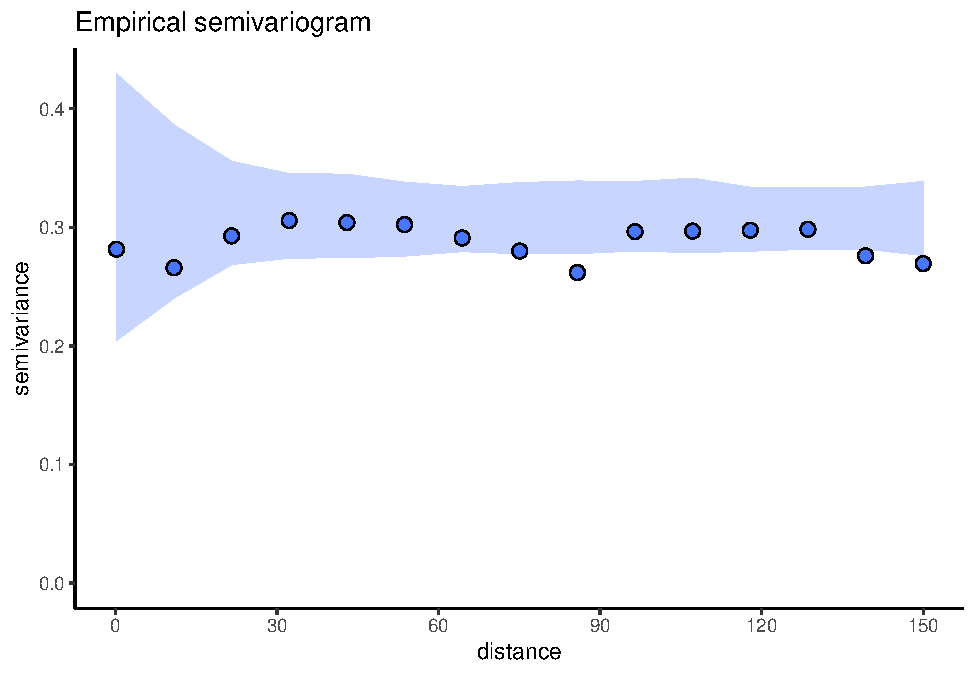
\includegraphics{skeleton_files/figure-latex/mixed_model-1.pdf}

\hypertarget{geostatistical-model}{%
\section{Geostatistical model}\label{geostatistical-model}}

We improve equation (1) by replacing the cluster level random effects
with a spatial gaussian process and we fit the following geostatistical
model \begin{equation}
Y_j(x_i)=\alpha+\gamma d_{ij} + \beta d(x_i) + S(x_{i}) + Z_{ij}
\end{equation}

\begin{Shaded}
\begin{Highlighting}[]
\NormalTok{fit_geo <-}\StringTok{ }\KeywordTok{linear.model.MLE}\NormalTok{(}\DataTypeTok{formula =}\NormalTok{ f,}
                            \DataTypeTok{coords =} \OperatorTok{~}\StringTok{ }\NormalTok{utm_x }\OperatorTok{+}\StringTok{ }\NormalTok{utm_y, }
                            \DataTypeTok{ID.coords =}\NormalTok{ haz}\OperatorTok{$}\NormalTok{ID,}
                            \DataTypeTok{data =}\NormalTok{ haz,}
                            \DataTypeTok{start.cov.pars =} \KeywordTok{c}\NormalTok{(}\DecValTok{15}\NormalTok{, }\FloatTok{0.2}\NormalTok{),}
                            \DataTypeTok{fixed.rel.nugget =} \DecValTok{0}\NormalTok{, }\DataTypeTok{kappa =} \FloatTok{0.5}\NormalTok{, }\DataTypeTok{method =} \StringTok{"nlminb"}\NormalTok{, }
                            \DataTypeTok{messages =}\NormalTok{ F)}
\KeywordTok{summary}\NormalTok{(fit_geo, }\DataTypeTok{l =}\NormalTok{ F)}
\end{Highlighting}
\end{Shaded}

\begin{verbatim}
## Geostatistical linear model 
## Call: 
## linear.model.MLE(formula = f, coords = ~utm_x + utm_y, data = haz, 
##     ID.coords = haz$ID, kappa = 0.5, fixed.rel.nugget = 0, start.cov.pars = c(15, 
##         0.2), method = "nlminb", messages = F)
## 
##                                       Estimate      StdErr  z.value
## (Intercept)                        -9.8061e-01  9.2504e-01  -1.0601
## agem                               -1.0697e-01  7.9639e-03 -13.4320
## I((agem - 17.84) * (agem > 17.84))  1.2104e-01  9.0655e-03  13.3513
## log_VITA                            1.4999e-01  8.5703e-02   1.7501
## elevation                           8.4161e-06  2.5432e-04   0.0331
## slope                              -4.5142e-02  1.9029e-02  -2.3722
## evi                                -4.6413e-01  5.2740e-01  -0.8800
##                                    p.value    
## (Intercept)                        0.28911    
## agem                               < 2e-16 ***
## I((agem - 17.84) * (agem > 17.84)) < 2e-16 ***
## log_VITA                           0.08010 .  
## elevation                          0.97360    
## slope                              0.01768 *  
## evi                                0.37884    
## ---
## Signif. codes:  0 '***' 0.001 '**' 0.01 '*' 0.05 '.' 0.1 ' ' 1
## 
## Log-likelihood: -2719.623
##  
## Covariance parameters Matern function 
## (fixed relative variance tau^2/sigma^2= 0) 
##         Estimate StdErr
## sigma^2  0.50264 0.1831
## phi      0.85266 0.8025
## omega^2  1.38995 0.2525
## 
## Legend: 
## sigma^2 = variance of the Gaussian process 
## phi = scale of the spatial correlation 
## omega^2 = variance of the individual unexplained variation
\end{verbatim}

\begin{Shaded}
\begin{Highlighting}[]
\CommentTok{# Save the results}
\CommentTok{# saveRDS(fit_geo, file = "output/fit_geo_070220.rds")}
\end{Highlighting}
\end{Shaded}

\hypertarget{predictions}{%
\section{Predictions}\label{predictions}}

\begin{Shaded}
\begin{Highlighting}[]
\CommentTok{# Extract values of covariates at prediction locations}
\NormalTok{cov_pred <-}\StringTok{ }\KeywordTok{extract}\NormalTok{(covariates, pred}\OperatorTok{$}\NormalTok{coords)}
\NormalTok{cov_pred <-}\StringTok{ }\KeywordTok{as.data.frame}\NormalTok{(cov_pred)}
\KeywordTok{names}\NormalTok{(cov_pred) <-}\StringTok{ }\KeywordTok{c}\NormalTok{(}\StringTok{"elevation"}\NormalTok{, }\StringTok{"slope"}\NormalTok{, }\StringTok{"evi"}\NormalTok{)}

\NormalTok{cov_pred}\OperatorTok{$}\NormalTok{agem <-}\StringTok{ }\KeywordTok{mean}\NormalTok{(haz}\OperatorTok{$}\NormalTok{agem)}
\NormalTok{cov_pred}\OperatorTok{$}\NormalTok{log_VITA <-}\StringTok{ }\KeywordTok{mean}\NormalTok{(haz}\OperatorTok{$}\NormalTok{log_VITA)}

\CommentTok{# Generate distribution of predictors at individual level}
\NormalTok{nsim <-}\StringTok{ }\DecValTok{1000}

\CommentTok{# Create function to sample from age}
\NormalTok{sample_age <-}\StringTok{ }\ControlFlowTok{function}\NormalTok{(nsim) \{}
\NormalTok{  t.age <-}\StringTok{ }\NormalTok{haz}\OperatorTok{$}\NormalTok{agem}
\NormalTok{  bw <-}\StringTok{ }\KeywordTok{density}\NormalTok{(t.age)}\OperatorTok{$}\NormalTok{bw}
\NormalTok{  t.age.obs <-}\StringTok{ }\NormalTok{t.age[}\KeywordTok{sample}\NormalTok{(}\DecValTok{1}\OperatorTok{:}\KeywordTok{nrow}\NormalTok{(haz), nsim, }\DataTypeTok{replace =} \OtherTok{TRUE}\NormalTok{)]}
\NormalTok{  t.age.sim <-}\StringTok{ }\KeywordTok{rnorm}\NormalTok{(n.sim,}\DataTypeTok{mean=}\NormalTok{t.age.obs,}\DataTypeTok{sd=}\NormalTok{bw)}
  \DecValTok{5}\OperatorTok{*}\KeywordTok{exp}\NormalTok{(t.age.sim)}\OperatorTok{/}\NormalTok{(}\DecValTok{1}\OperatorTok{+}\KeywordTok{exp}\NormalTok{(t.age.sim))}
\NormalTok{\}}

\CommentTok{# Obtain predictions}
\NormalTok{predictions <-}\StringTok{ }\KeywordTok{spatial.pred.linear.MLE}\NormalTok{(fit_geo, }
                                       \DataTypeTok{grid.pred =}\NormalTok{ pred}\OperatorTok{$}\NormalTok{coords, }
                                       \DataTypeTok{predictors =}\NormalTok{ cov_pred, }
                                       \DataTypeTok{n.sim.prev =}\NormalTok{ nsim,}
                                       \DataTypeTok{scale.predictions =} \StringTok{"logit"}\NormalTok{,}
                                       \CommentTok{# type="joint",}
                                       \DataTypeTok{thresholds =} \DecValTok{-2}\NormalTok{,}
                                       \DataTypeTok{scale.thresholds =} \StringTok{"logit"}\NormalTok{)}
\end{Highlighting}
\end{Shaded}

\begin{verbatim}
## NOTE: the nugget effect IS NOT included in the predictions. 
## Type of prevalence predictions: marginal 
## Spatial predictions: logit
\end{verbatim}

\begin{Shaded}
\begin{Highlighting}[]
\NormalTok{predictions}\OperatorTok{$}\NormalTok{exceedance.prob <-}\StringTok{ }\DecValTok{1} \OperatorTok{-}\StringTok{ }\NormalTok{predictions}\OperatorTok{$}\NormalTok{exceedance.prob}

\CommentTok{# Save predictions}
\CommentTok{# saveRDS(predictions, "output/geo_pred_070220.rds")}
\end{Highlighting}
\end{Shaded}

\begin{Shaded}
\begin{Highlighting}[]
\NormalTok{haz_pred <-}\StringTok{ }\KeywordTok{rasterFromXYZ}\NormalTok{(}\KeywordTok{data.frame}\NormalTok{(pred}\OperatorTok{$}\NormalTok{coords, }
                                     \DataTypeTok{haz =}\NormalTok{ predictions}\OperatorTok{$}\NormalTok{logit}\OperatorTok{$}\NormalTok{predictions,}
                                     \DataTypeTok{pstunting =} \KeywordTok{as.numeric}\NormalTok{(predictions}\OperatorTok{$}\NormalTok{exceedance.prob)))}

\KeywordTok{tm_shape}\NormalTok{(haz_pred) }\OperatorTok{+}
\StringTok{  }\KeywordTok{tm_raster}\NormalTok{(}\DataTypeTok{col =} \StringTok{"haz"}\NormalTok{, }\DataTypeTok{palette =} \StringTok{"RdYlBu"}\NormalTok{, }\DataTypeTok{legend.show =}\NormalTok{ T, }\DataTypeTok{style =} \StringTok{"cont"}\NormalTok{,}
            \DataTypeTok{title =} \StringTok{"Predicted mean HAZ"}\NormalTok{) }\OperatorTok{+}
\KeywordTok{tm_shape}\NormalTok{(uga, }\DataTypeTok{is.master =}\NormalTok{ T,) }\OperatorTok{+}
\StringTok{  }\KeywordTok{tm_borders}\NormalTok{(}\StringTok{"black"}\NormalTok{, }\DataTypeTok{lwd =} \DecValTok{1}\NormalTok{) }\OperatorTok{+}
\StringTok{  }\KeywordTok{tm_compass}\NormalTok{(}\DataTypeTok{position =} \KeywordTok{c}\NormalTok{(}\StringTok{"right"}\NormalTok{, }\StringTok{"top"}\NormalTok{)) }\OperatorTok{+}
\StringTok{  }\KeywordTok{tm_scale_bar}\NormalTok{(}\DataTypeTok{position =} \KeywordTok{c}\NormalTok{(}\StringTok{"right"}\NormalTok{, }\StringTok{"bottom"}\NormalTok{)) }\OperatorTok{+}
\StringTok{  }\KeywordTok{tm_layout}\NormalTok{(}\DataTypeTok{design.mode =}\NormalTok{ F, }\DataTypeTok{legend.bg.color =} \StringTok{"white"}\NormalTok{, }\DataTypeTok{scale =} \FloatTok{1.2}\NormalTok{,}
            \DataTypeTok{legend.position =} \KeywordTok{c}\NormalTok{(}\StringTok{"left"}\NormalTok{, }\StringTok{"top"}\NormalTok{), }\DataTypeTok{frame =}\NormalTok{ T, }\DataTypeTok{outer.margins =} \DecValTok{0}\NormalTok{, }\DataTypeTok{asp =} \DecValTok{0}\NormalTok{) }
\end{Highlighting}
\end{Shaded}

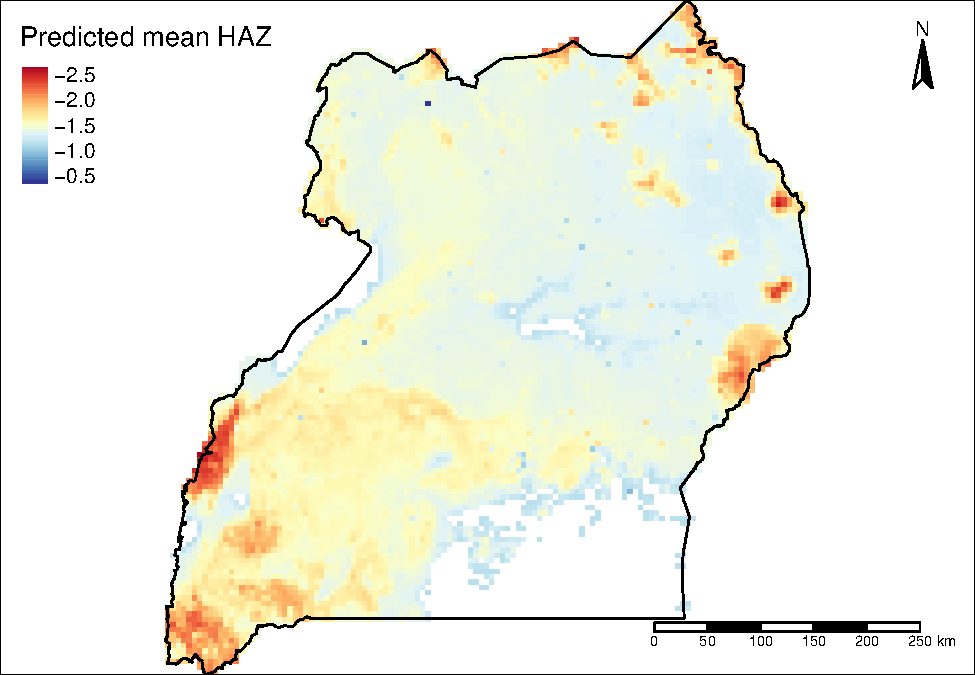
\includegraphics{skeleton_files/figure-latex/maps-1.pdf}

\begin{Shaded}
\begin{Highlighting}[]
\NormalTok{pal_ex <-}\StringTok{ }\NormalTok{tmaptools}\OperatorTok{::}\KeywordTok{get_brewer_pal}\NormalTok{(}\StringTok{"-RdYlBu"}\NormalTok{, }\DataTypeTok{n =} \DecValTok{10}\NormalTok{, }\DataTypeTok{contrast =} \KeywordTok{c}\NormalTok{(}\DecValTok{0}\NormalTok{, }\DecValTok{1}\NormalTok{), }\DataTypeTok{plot =}\NormalTok{ F)}

\KeywordTok{tm_shape}\NormalTok{(haz_pred) }\OperatorTok{+}
\StringTok{  }\KeywordTok{tm_raster}\NormalTok{(}\DataTypeTok{col =} \StringTok{"pstunting"}\NormalTok{, }\DataTypeTok{palette =}\NormalTok{ pal_ex, }\DataTypeTok{legend.show =}\NormalTok{ F,}
            \DataTypeTok{style =} \StringTok{"fixed"}\NormalTok{, }\DataTypeTok{breaks =} \KeywordTok{seq}\NormalTok{(}\DecValTok{0}\NormalTok{, }\DecValTok{1}\NormalTok{, }\DataTypeTok{by =} \FloatTok{.1}\NormalTok{)) }\OperatorTok{+}
\StringTok{  }\KeywordTok{tm_add_legend}\NormalTok{(}\DataTypeTok{type =} \StringTok{"fill"}\NormalTok{,}
                \DataTypeTok{labels =} \KeywordTok{c}\NormalTok{(}\StringTok{"0 - 0.1"}\NormalTok{, }\StringTok{"0.1 - 0.2"}\NormalTok{, }\StringTok{"0.2 - 0.3"}\NormalTok{, }\StringTok{"0.3 - 0.4"}\NormalTok{, }\StringTok{"0.4 - 0.5"}\NormalTok{,}
                         \StringTok{"0.5 - 0.6"}\NormalTok{, }\StringTok{"0.6 - 0.7"}\NormalTok{, }\StringTok{"0.7 - 0.8"}\NormalTok{, }\StringTok{"0.8 - 0.9"}\NormalTok{, }\StringTok{"0.9 - 1"}\NormalTok{),}
                \DataTypeTok{col =}\NormalTok{ pal_ex, }\DataTypeTok{size =} \FloatTok{.5}\NormalTok{, }\DataTypeTok{alpha =} \DecValTok{1}\NormalTok{,}
                \DataTypeTok{title =} \StringTok{"Probability of}\CharTok{\textbackslash{}n}\StringTok{stunting"}\NormalTok{,}
                \DataTypeTok{is.portrait =}\NormalTok{ T) }\OperatorTok{+}
\KeywordTok{tm_shape}\NormalTok{(uga, }\DataTypeTok{is.master =}\NormalTok{ T,) }\OperatorTok{+}
\StringTok{  }\KeywordTok{tm_borders}\NormalTok{(}\StringTok{"black"}\NormalTok{, }\DataTypeTok{lwd =} \DecValTok{1}\NormalTok{) }\OperatorTok{+}
\StringTok{  }\KeywordTok{tm_compass}\NormalTok{(}\DataTypeTok{position =} \KeywordTok{c}\NormalTok{(}\StringTok{"right"}\NormalTok{, }\StringTok{"top"}\NormalTok{)) }\OperatorTok{+}
\StringTok{  }\KeywordTok{tm_scale_bar}\NormalTok{(}\DataTypeTok{position =} \KeywordTok{c}\NormalTok{(}\StringTok{"right"}\NormalTok{, }\StringTok{"bottom"}\NormalTok{)) }\OperatorTok{+}
\StringTok{  }\KeywordTok{tm_layout}\NormalTok{(}\DataTypeTok{design.mode =}\NormalTok{ F, }\DataTypeTok{legend.bg.color =} \StringTok{"white"}\NormalTok{, }\DataTypeTok{scale =} \FloatTok{1.2}\NormalTok{,}
            \DataTypeTok{legend.position =} \KeywordTok{c}\NormalTok{(}\StringTok{"left"}\NormalTok{, }\StringTok{"top"}\NormalTok{), }\DataTypeTok{frame =}\NormalTok{ T, }\DataTypeTok{outer.margins =} \DecValTok{0}\NormalTok{, }\DataTypeTok{asp =} \DecValTok{0}\NormalTok{)}
\end{Highlighting}
\end{Shaded}

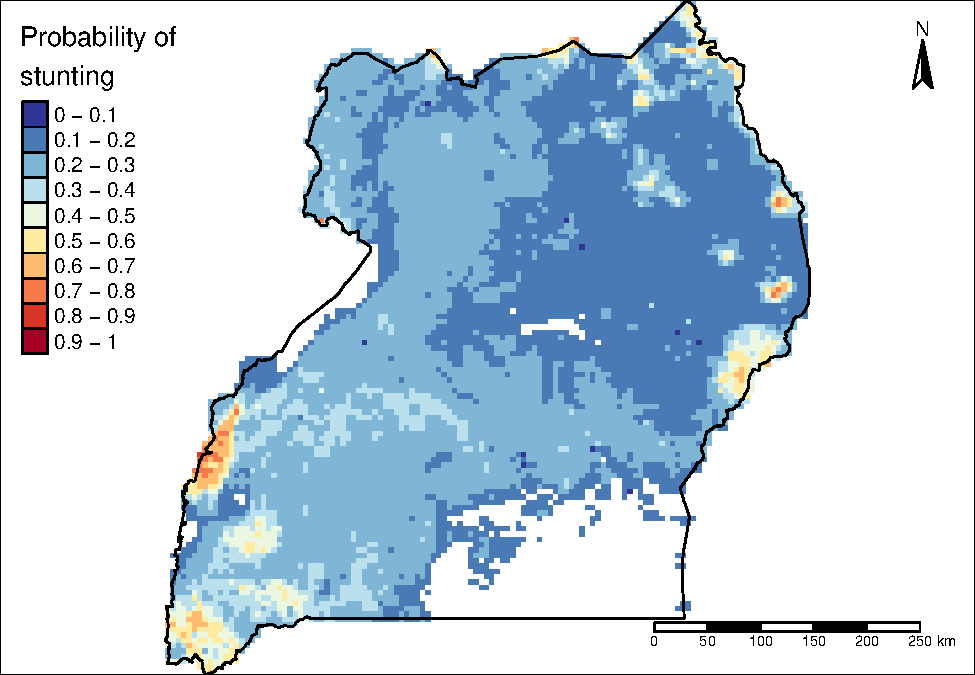
\includegraphics{skeleton_files/figure-latex/maps-2.pdf}




\newpage
\singlespacing 
\bibliography{biblio.bib}

\end{document}
